\documentclass[11pt,a4paper]{article}
\usepackage[a4paper,margin=0.72in]{geometry}
\usepackage[T1]{fontenc}
\usepackage[utf8]{inputenc}
\usepackage{newtxtext,newtxmath}
\usepackage{graphicx}
\usepackage{booktabs}
\usepackage{array}
\usepackage{float}
\usepackage{microtype}
\usepackage{setspace}
\usepackage[hidelinks]{hyperref}
\usepackage{caption}
\usepackage[numbers,sort&compress]{natbib}
\usepackage{xcolor}
\usepackage{tikz}
\usetikzlibrary{arrows.meta,positioning,shapes.geometric,fit,backgrounds,calc}
\usepackage{fancyhdr}
\usepackage{titlesec}
\definecolor{navy}{HTML}{17324D}
\definecolor{teal}{HTML}{147D78}
\definecolor{pale}{HTML}{EAF2F8}
\definecolor{mint}{HTML}{E7F4F1}
\definecolor{gold}{HTML}{F7EED8}
\definecolor{rose}{HTML}{F8E9E7}
\definecolor{slate}{HTML}{526477}
\pagestyle{fancy}
\fancyhf{}
\fancyhead[L]{\footnotesize MARP: Model-Aware Readiness}
\fancyhead[R]{\footnotesize FACEATTEND engineering case study}
\fancyfoot[C]{\thepage}
\renewcommand{\headrulewidth}{0.4pt}
\renewcommand{\footrulewidth}{0pt}
\setlength{\headheight}{14pt}
\titleformat{\section}{\large\bfseries\color{navy}}{\thesection}{0.6em}{}
\titleformat{\subsection}{\normalsize\bfseries\color{teal}}{\thesubsection}{0.6em}{}
\setlength{\parindent}{0pt}
\setlength{\parskip}{4pt}
\setstretch{1.03}
\captionsetup{font=small,labelfont=bf}
\renewcommand{\arraystretch}{1.18}
\title{\textbf{MARP: A Model-Aware Readiness Protocol with In-Situ Chaos Engineering for Edge AI Microservices}}
\author{\textbf{Mellamarthi Mithilesh}\\
\small Department of Computer Science and Engineering, KL University, Vijayawada, Andhra Pradesh, India}
\date{November 25, 2026}
\begin{document}
\maketitle

\textbf{Abstract.} AI-enabled services can appear operational while required models are still initializing or a critical dependency is unavailable. In such conditions, a process-level health check may not be sufficient to determine whether a service should receive requests. This paper presents an engineering case study of the Model-Aware Readiness Protocol (MARP) within FACEATTEND, a web-based attendance prototype built with React, FastAPI, PostgreSQL and Docker Compose. The approach treats readiness as an application-level condition that depends on database availability and completion of computer-vision initialization, and pairs readiness reporting with selected fault-testing and telemetry mechanisms. The manuscript synthesizes the system design and previously reported verification evidence. A November 2026 verification gate re-executed the full backend suite (169 passed), the configuration suite (25 passed), and the browser suite (59 passed) against the redesigned interface, rebuilt the frontend production bundle successfully, and verified template-packaging checks including compose rendering and white-label builds; earlier phases additionally described a database-initialization race test using four independent processes. These figures demonstrate reported software-verification coverage, not empirical gains in startup latency, recovery time, face-recognition accuracy or user capacity. The paper therefore defines a reproducible evaluation protocol for measuring readiness correctness, time to readiness, recovery latency and monitoring overhead under controlled dependency and model failures. The contribution is a transparent implementation case study and an evaluation plan, with empirical performance claims reserved until controlled measurements are collected.

\textbf{Keywords:} Model-aware readiness; chaos engineering; edge AI; microservices; attendance systems

\section{Introduction}

Computer-vision services are not ready merely because their process has started or an HTTP port is accepting connections. Before a request can be handled correctly, the service may need to establish database access, load model weights, allocate memory, initialize libraries and prepare dependent components. If traffic reaches the application before these steps complete, users can observe avoidable errors, timeouts or inconsistent behaviour. This distinction matters in resource-constrained and edge-oriented deployments, where initialization can be a meaningful part of the service lifecycle.

Operational health signals serve different purposes. A startup probe allows a component time to initialize; a liveness probe helps identify a process that should be restarted; and a readiness probe indicates whether an instance should receive the requests it advertises as able to handle. Kubernetes documents these as separate probe mechanisms rather than interchangeable checks \cite{Kubernetes}. For a machine-learning service, readiness may need to include application-specific conditions beyond a live process, such as successful loading of a required detector and access to the data store used by the request path.

This paper examines that problem through FACEATTEND, a college attendance prototype with a web frontend, API backend, database, computer-vision processing and an application-level readiness component referred to as the Model-Aware Readiness Protocol (MARP). The paper focuses on service reliability, not on claiming that the current face matcher achieves a particular recognition accuracy. The reported matching baseline uses a normalized 64 × 64 grayscale image represented as a 4,096-value vector and nearest-template Euclidean distance with a default threshold reported as 0.85. In the absence of a labelled evaluation dataset and threshold calibration, that pipeline must be treated as a baseline implementation rather than a validated biometric recognizer.

The central question is practical: how can the service communicate that its critical dependencies and model initialization are ready, and how can that behaviour be tested when a dependency or initialization step fails? This question aligns with broader work on the operational complexity of machine-learning systems \cite{Sculley,Amershi} and with chaos engineering, which uses controlled experiments to learn how a system behaves under failure \cite{Basiri}.

\subsection{Objectives and research questions}

The study has three objectives: (i) describe a model-aware readiness design for an AI-enabled attendance service; (ii) distinguish implemented or previously reported verification evidence from behaviour that remains unmeasured; and (iii) define a reproducible experiment for testing readiness, fault response and recovery. The following questions guide the evaluation:

RQ1: Does model- and dependency-aware readiness prevent a service from reporting READY while a required initialization or database condition is unmet?

RQ2: How do controlled model-initialization delays and database failures affect readiness transitions and request outcomes?

RQ3: What are the time-to-ready, recovery latency and monitoring overhead under repeatable test conditions?

\subsection{Research gap and contribution}

The research gap is framed narrowly. General-purpose orchestration probes provide useful lifecycle controls, while machine-learning engineering research emphasizes the additional operational burden created by models, data dependencies and model-serving pipelines \cite{Breck,Amershi}. Chaos-engineering approaches provide methods for controlled failure experiments \cite{Basiri}, but a project still needs to connect those experiments to its own application state and define what constitutes a correct readiness response. This case study addresses that implementation-level gap by documenting a readiness contract tied to the attendance service’s critical dependencies and by setting out measurements that can test whether the contract works. It does not claim to be the first model-aware readiness system or to establish novelty across all prior work.

The paper contributes (1) a system-level account of MARP in a real software prototype, (2) a traceable summary of the project’s reported automated verification, (3) an explicit boundary between simulated fault controls and actual dependency failure, and (4) a repeatable evaluation protocol for the next experimental stage.

\section{Design/Methods/Modelling}

\subsection{Study design and system architecture}

The work is an engineering case study with a preliminary verification review. It uses the project architecture, recorded implementation notes and a prior R11 audit summary as sources of evidence. The test counts presented later are reported results from that audit, not fresh executions performed for this manuscript. The study does not use student face images as an experimental dataset and does not make statistical claims about recognition performance.

FACEATTEND is described as a React 18 web interface backed by a Python FastAPI service, SQLAlchemy persistence, PostgreSQL and Docker Compose. Docker Compose is the documented local multi-container orchestration approach in the reviewed project materials. The architecture separates the browser client, API service, persistent database and computer-vision request path. Kubernetes is relevant as a possible deployment target because its startup, readiness and liveness probes provide distinct lifecycle controls; however, a successful Kubernetes deployment is not established by the evidence reviewed here and is not presented as an implemented or validated project result. The reported feature inventory includes role-oriented login screens, student enrollment, attendance sessions, a camera/WebSocket path, an HTTP image-detection path, attendance summaries, student views and telemetry export. These are product-level workflows; each should be rechecked in the exact demonstration environment before a claim is made about live operation.

\begin{figure}[H]
\centering
\resizebox{\linewidth}{!}{%
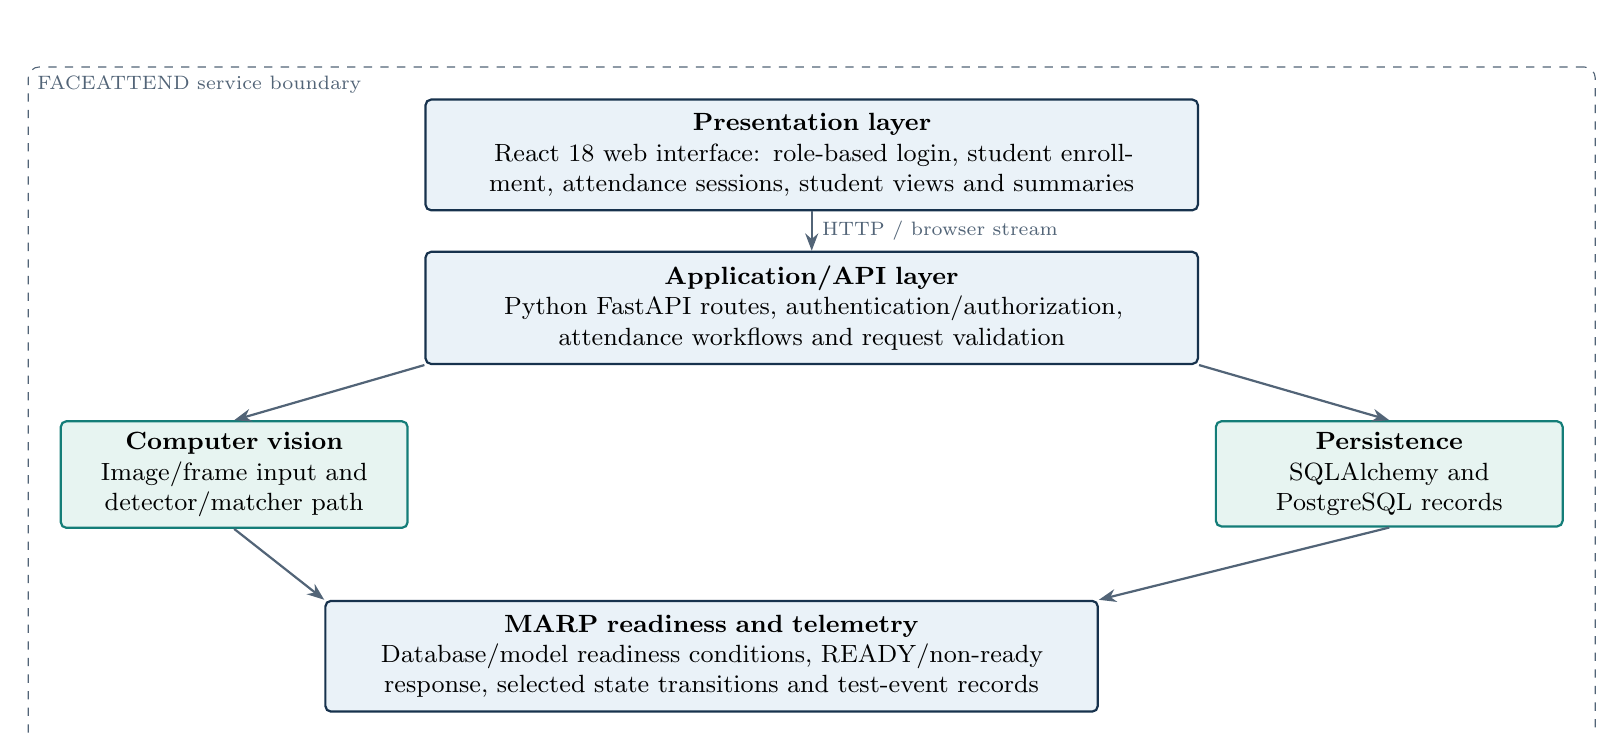
\begin{tikzpicture}[
  node distance=5mm and 7mm,
  block/.style={draw=navy, rounded corners=2pt, line width=0.8pt, fill=pale,
    align=center, text width=0.78\linewidth, minimum height=8mm, inner sep=5pt, font=\small},
  service/.style={draw=teal, rounded corners=2pt, line width=0.8pt, fill=mint,
    align=center, text width=0.34\linewidth, minimum height=12mm, inner sep=4pt, font=\small},
  arrow/.style={-{Stealth[length=2.2mm]}, line width=0.8pt, draw=slate}
]
\node[block] (client) {\textbf{Presentation layer}\\React 18 web interface: role-based login, student enrollment, attendance sessions, student views and summaries};
\node[block, below=of client] (api) {\textbf{Application/API layer}\\Python FastAPI routes, authentication/authorization, attendance workflows and request validation};
\node[service, below left=7mm and 2mm of api] (vision) {\textbf{Computer vision}\\Image/frame input and detector/matcher path};
\node[service, below right=7mm and 2mm of api] (db) {\textbf{Persistence}\\SQLAlchemy and PostgreSQL records};
\node[block, below=9mm of vision, xshift=0.5\linewidth] (marp) {\textbf{MARP readiness and telemetry}\\Database/model readiness conditions, READY/non-ready response, selected state transitions and test-event records};
\draw[arrow] (client) -- node[right,font=\scriptsize,text=slate]{HTTP / browser stream} (api);
\draw[arrow] (api.south west) -- (vision.north);
\draw[arrow] (api.south east) -- (db.north);
\draw[arrow] (vision.south) -- (marp.north west);
\draw[arrow] (db.south) -- (marp.north east);
\node[draw=slate,dashed,rounded corners,fit=(client)(api)(vision)(db)(marp),inner sep=4mm] (system) {};
\node[anchor=north west,font=\scriptsize\color{slate}] at (system.north west) {FACEATTEND service boundary};
\end{tikzpicture}}
\caption{Conceptual FACEATTEND architecture and MARP readiness/telemetry path.}
\label{fig:architecture}
\end{figure}

At the service layer, the browser sends requests to FastAPI. The API uses PostgreSQL for persistent records and invokes computer-vision processing for attendance-related requests. MARP provides a separate readiness signal and a place to record state transitions or selected test events. This separation is important: application readiness indicates whether the relevant request path is prepared; it does not establish that recognition decisions are accurate or that the system can sustain a specified number of concurrent users.

\subsection{Model-Aware Readiness Protocol}

The audited design describes readiness as a state rather than a simple process-alive flag. During startup, the service checks the database condition and initializes the required detector/model path under a bounded initialization process. The reported readiness endpoint returns HTTP 200 when the required conditions are ready and HTTP 503 while the service is loading or has a recorded readiness failure. The documented state reasons include database, model, timeout and busy conditions. These behaviours should be verified against the release candidate before publication because the manuscript is based on recorded project evidence rather than a fresh source-code audit.

The conceptual contract is: (1) initialize the process; (2) validate required database access; (3) initialize or validate the required vision component; (4) transition to READY only when both dependencies satisfy the defined conditions; and (5) return a non-ready status with a diagnostic reason if a required step fails. A recovery action or restart should return the service to an explicitly defined path rather than silently treating a previous failure as success. Concurrent first-time initializers serialize schema creation through a transaction-scoped PostgreSQL advisory lock (applied only on PostgreSQL deployments), so a second initializer waits and then no-ops on the existing schema. Figure 2 summarizes this model; it is a conceptual workflow and not a measured state-transition trace.

\begin{figure}[H]
\centering
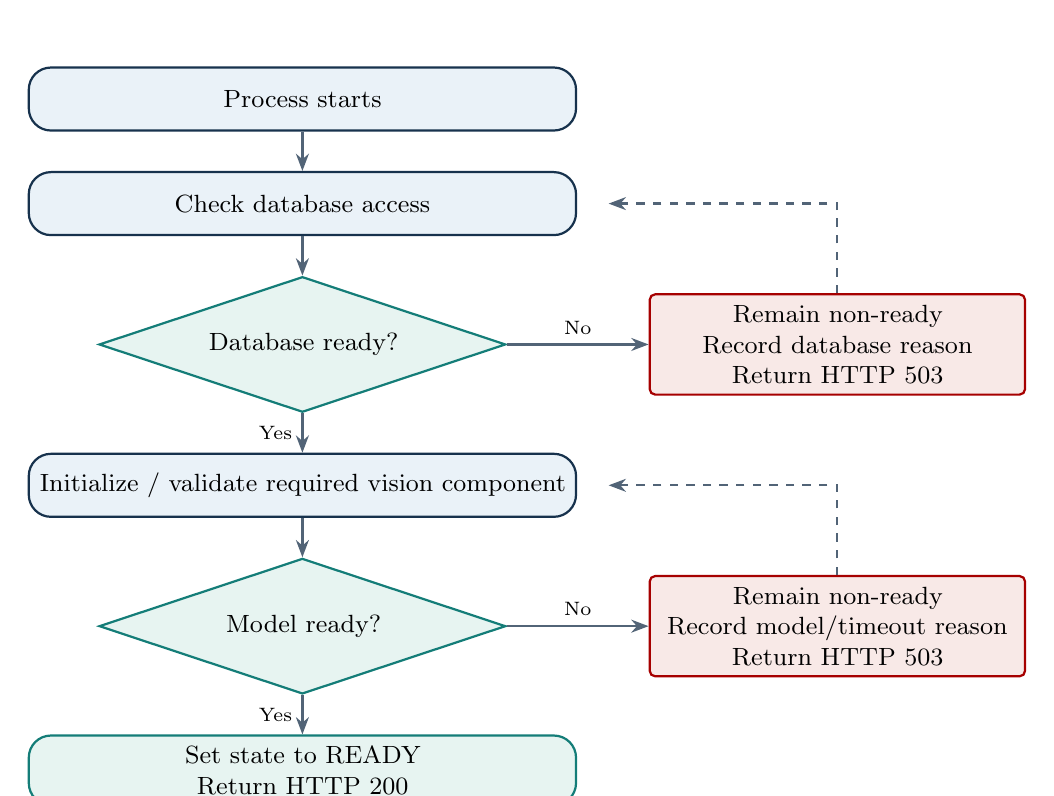
\begin{tikzpicture}[
  node distance=5mm,
  startstop/.style={draw=navy, rounded corners=8pt, fill=pale, line width=0.8pt,
    align=center, text width=0.55\linewidth, minimum height=8mm, inner sep=4pt, font=\small},
  decision/.style={diamond, aspect=3.0, draw=teal, fill=mint, line width=0.8pt,
    align=center, text width=0.31\linewidth, inner sep=2pt, font=\small},
  fail/.style={draw=red!65!black, rounded corners=2pt, fill=rose, line width=0.8pt,
    align=center, text width=0.37\linewidth, minimum height=9mm, inner sep=4pt, font=\small},
  arrow/.style={-{Stealth[length=2.2mm]}, line width=0.8pt, draw=slate}
]
\node[startstop] (start) {Process starts};
\node[startstop, below=of start] (db) {Check database access};
\node[decision, below=of db] (dbok) {Database ready?};
\node[startstop, below=of dbok] (model) {Initialize / validate required vision component};
\node[decision, below=of model] (modelok) {Model ready?};
\node[startstop, below=of modelok, fill=mint, draw=teal] (ready) {Set state to READY\\Return HTTP 200};
\node[fail, right=18mm of dbok] (dbfail) {Remain non-ready\\Record database reason\\Return HTTP 503};
\node[fail, right=18mm of modelok] (mfail) {Remain non-ready\\Record model/timeout reason\\Return HTTP 503};
\draw[arrow] (start) -- (db);
\draw[arrow] (db) -- (dbok);
\draw[arrow] (dbok) -- node[left,font=\scriptsize]{Yes} (model);
\draw[arrow] (dbok.east) -- node[above,font=\scriptsize]{No} (dbfail.west);
\draw[arrow] (model) -- (modelok);
\draw[arrow] (modelok) -- node[left,font=\scriptsize]{Yes} (ready);
\draw[arrow] (modelok.east) -- node[above,font=\scriptsize]{No} (mfail.west);
\draw[arrow,dashed] (dbfail.north) |- ([xshift=4mm]db.east);
\draw[arrow,dashed] (mfail.north) |- ([xshift=4mm]model.east);
\end{tikzpicture}
\caption{Conceptual MARP readiness decision flow. Failure branches remain non-ready until recovery is explicitly validated; this diagram describes the intended contract, not a measured trace.}
\label{fig:readiness}
\end{figure}

This design is intended to reduce false-ready windows: the interval in which an instance appears available to the orchestration or caller while a required component is not yet usable. The protocol is not an automatic repair mechanism. A 503 response can communicate unavailability, but it does not fix the dependency, correct a model defect or guarantee that a gateway will recover without correct routing and timeout configuration.

\subsection{Fault testing and telemetry}

Fault injection is useful only when the injected event, expected behaviour and observed result are explicit. The project notes describe controls for selected readiness and dependency scenarios, as well as a separate test harness that can interrupt a disposable database during initialization and check for a non-ready response followed by recovery. Earlier audit notes also indicate that some user-interface controls simulate state changes rather than causing an underlying infrastructure fault. For that reason, the study classifies tests by what they actually manipulate; it does not treat every interface control as proof of a real database outage or model crash.

A controlled test should record the initial state, trigger, expected readiness outcome, actual HTTP status, state reason, application logs, timestamp of fault introduction, timestamp of fault removal and timestamp at which readiness becomes stable again. Telemetry can help preserve this sequence for later analysis. Telemetry volume alone is not a reliability outcome: the data must be complete enough to reconstruct the event and its relationship to the readiness signal.

\begin{figure}[H]
\centering
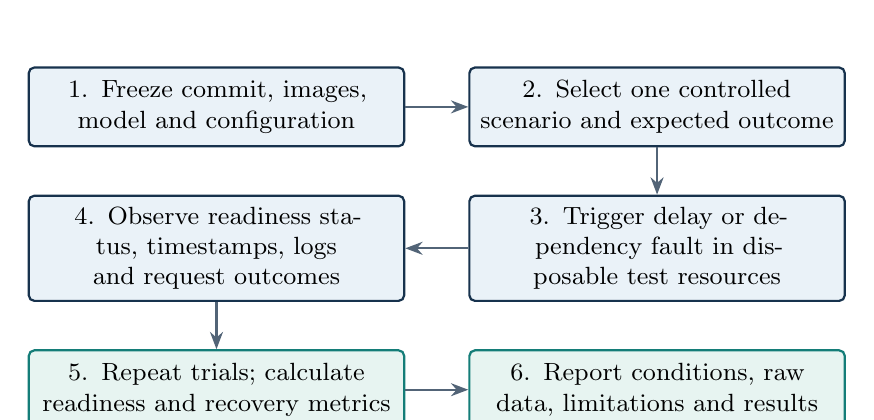
\begin{tikzpicture}[
  node distance=6mm and 8mm,
  workflowbox/.style={draw=navy, rounded corners=2pt, fill=pale, line width=0.8pt,
    align=center, text width=0.37\linewidth, minimum height=10mm, inner sep=4pt, font=\small},
  evidencebox/.style={draw=teal, rounded corners=2pt, fill=mint, line width=0.8pt,
    align=center, text width=0.37\linewidth, minimum height=10mm, inner sep=4pt, font=\small},
  arrow/.style={-{Stealth[length=2.2mm]}, line width=0.8pt, draw=slate}
]
\node[workflowbox] (freeze) {1. Freeze commit, images, model and configuration};
\node[workflowbox, right=of freeze] (scenario) {2. Select one controlled scenario and expected outcome};
\node[workflowbox, below=of scenario] (inject) {3. Trigger delay or dependency fault in disposable test resources};
\node[workflowbox, left=of inject] (observe) {4. Observe readiness status, timestamps, logs and request outcomes};
\node[evidencebox, below=of observe] (analyse) {5. Repeat trials; calculate readiness and recovery metrics};
\node[evidencebox, right=of analyse] (report) {6. Report conditions, raw data, limitations and results};
\draw[arrow] (freeze) -- (scenario);
\draw[arrow] (scenario) -- (inject);
\draw[arrow] (inject) -- (observe);
\draw[arrow] (observe) -- (analyse);
\draw[arrow] (analyse) -- (report);
\end{tikzpicture}
\caption{Proposed reproducible fault-evaluation workflow. This is a protocol for future measurement, not a claim that the experiment has already been completed.}
\label{fig:experiment}
\end{figure}

\subsection{Experimental procedure for empirical evaluation}

A controlled comparative experiment remains necessary to answer RQ1–RQ3 quantitatively. The following protocol is specified for execution; its measurements are not presented as completed results in this paper.

\begin{enumerate}

\item Freeze the software commit, container image identifiers, dependency versions, model files, hardware, operating system and relevant configuration. Save the configuration and logs for each run.

\item Define a baseline readiness check and the MARP condition being compared. Use the same machine, database snapshot, request mix and model for each condition; change one factor at a time.

\item Run a normal-start scenario, a controlled model-initialization delay, a database-unavailable-at-startup scenario, a database interruption after READY, and a model-initialization failure. Test recovery after restoring the dependency. Execute destructive fault scenarios only against disposable test resources.

\item Repeat each scenario at least 30 times where the environment permits, randomize or alternate baseline and MARP run order, and report exclusions. Record timestamps with a monotonic clock and retain raw JSON/CSV outputs.

\item Calculate time-to-ready, false-ready rate, request failures before readiness, recovery latency, p50/p95 request latency and resource overhead. Report medians and dispersion or confidence intervals, alongside the exact test conditions.

\item Run load testing as a separate experiment. Generate a predefined concurrency profile and report throughput, latency percentiles, error rate and resource usage. Do not infer capacity from unit tests or fault-injection tests.

\end{enumerate}

\textbf{Table 1. Proposed controlled scenarios and primary measurements.}

\begin{table}[H]\centering\small

\begin{tabular}{|p{0.23\linewidth}|p{0.29\linewidth}|p{0.36\linewidth}|}\hline

\textbf{Scenario} & \textbf{Expected behaviour to test} & \textbf{Measurements}\\\hline

Normal cold start & READY occurs only after required components pass checks. & Time-to-ready; initial errors.\\\hline

Delayed model init & Service remains not ready during model initialization. & False-ready rate; transition timestamps.\\\hline

Database unavailable & Readiness reports dependency failure; recovery is explicit. & 503/200 timeline; recovery latency.\\\hline

Model init failure & READY is withheld and failure reason is observable. & Readiness state; logs; retry/restart behaviour.\\\hline

Concurrent load & System degrades predictably and reports request outcomes. & Throughput; p50/p95 latency; error and resource rates.\\\hline

\end{tabular}\end{table}

\subsection{Outcome definitions and validity controls}

Time-to-ready is defined as the time between process start and the first valid READY transition. Recovery latency is the interval between restoration of a failed dependency and a stable READY state; stability should be defined in advance, for example as three consecutive successful readiness observations. False-ready rate is the proportion of probes or requests for which the service claims readiness while a required component is deliberately unavailable. All denominators and polling intervals must be reported. Using different probe intervals across conditions would confound the comparison.

Threats to validity include machine load variation, warm caches, different model binaries, nondeterministic network or database delays, stale containers, and fault controls that simulate status without interrupting the real dependency. A repeatable experiment must distinguish simulated-state tests from real dependency tests and preserve evidence for both. The current paper does not report empirical estimates because raw trial-level observations are not available in the reviewed materials.

\section{Results and Discussion}

\subsection{Previously reported verification evidence}

The prior project audit summary reports several software-verification results. These are included to make the current engineering maturity visible, but the evidence provenance is important: the backend, configuration, and browser suites below were re-executed in a November 2026 verification gate (all with exit code 0, including 59 browser tests against the redesigned interface), while fault-injection and latency figures remain reported-only. Results describe what was measured and should be reconfirmed against the final submission commit.

\textbf{Table 2. Verification evidence reported by the project audit.}

\begin{table}[H]\centering\small

\begin{tabular}{|p{0.23\linewidth}|p{0.29\linewidth}|p{0.36\linewidth}|}\hline

\textbf{Evidence item} & \textbf{Reported result} & \textbf{What it supports—and what it does not}\\\hline

Backend automated tests & 169 passed (re-executed Nov 2026, exit 0). & Supports regression coverage in the audited configuration; does not establish field reliability.\\\hline

Deployment/configuration tests & 25 passed (re-executed Nov 2026, exit 0). & Supports checks on environment and configuration rules; does not prove a production deployment.\\\hline

Browser tests & 59 Playwright tests passed (re-executed Nov 2026 against the redesigned interface, exit 0). & Supports tested browser flows; prior audit describes many API interactions as mocked.\\\hline

Frontend production build & Rebuilt successfully (Nov 2026). & Supports build reproducibility at that point; not equivalent to a full live deployment test.\\\hline

Database initialization race & Four independent processes used in a reported test with a PostgreSQL advisory lock. & Supports a targeted concurrency check; not a general load-capacity result.\\\hline

\end{tabular}\end{table}

Taken together, these reported checks indicate that the team has invested in route-level security, startup/configuration behaviour, regression testing and selected database initialization concurrency. The reported browser coverage is useful, but mocked API behaviour cannot demonstrate that the live camera stream, detector and database will work together under classroom conditions. Similarly, a test that validates the service returns 503 while a dependency is unavailable shows protocol behaviour for that scenario; it does not by itself quantify how much time is saved or whether all failure modes are handled.

\subsection{Interpretation against the research questions}

RQ1 is supported at the design and test-intent level: the audited design makes readiness conditional on model and database state and uses distinct READY and non-ready responses. However, without trial-level readiness-transition traces (the re-executed suites assert pass/fail behaviour, not transition timing), the manuscript cannot state a measured false-ready rate or prove the condition across every startup path. The empirical answer requires the controlled scenarios in Table 1.

RQ2 is only partially answered. The project reports fault-testing capabilities and a database-interruption harness, but the reviewed evidence does not include a trial-level dataset of readiness transitions, request errors or recovery durations. An implementation that returns 503 for a known injected fault is a useful correctness check; comparative evidence requires the baseline and MARP to be run under the same fault with repeated trials.

RQ3 remains open. There are no verified startup-time distributions, recovery-time distributions, monitoring-overhead measurements or concurrent-user capacity results in the material reviewed for this paper. This is not a cosmetic omission: those measurements are needed to justify claims that the protocol is faster, more reliable or more efficient. Reporting them as future work is scientifically stronger than substituting invented numbers or treating test counts as performance metrics.

\subsection{Computer-vision and deployment boundaries}

The attendance matcher also imposes a separate validity boundary. Learned face-recognition methods such as FaceNet \cite{Schroff} and ArcFace \cite{Deng} learn feature representations designed for identity comparison. The audited FACEATTEND baseline instead uses normalized grayscale pixel vectors and a nearest-template distance threshold reported as 0.85, with explicit rejection of missing, malformed, or non-finite template vectors before any comparison. These approaches are not equivalent. Because the threshold has not been calibrated on a labelled dataset, the paper does not claim accuracy, false-acceptance rate, false-rejection rate or demographic fairness. Robust liveness detection and resistance to presentation attacks are also not demonstrated.

The same discipline applies to deployment. Local Docker Compose verification does not prove successful Kubernetes deployment, operational monitoring in production or capacity for 100 or more concurrent users. Health endpoints, fault injection and load testing answer different questions: health endpoints communicate state; fault injection probes selected behaviour under a controlled failure; load testing estimates performance under a specified workload. A credible evaluation should report each separately.

\subsection{Practical implications}

For developers, an explicit readiness contract makes failure state visible and can prevent a caller or orchestrator from mistaking an initialized process for a usable AI service. For the project team, a written fault matrix and timestamped telemetry can convert an informal demonstration into a repeatable verification exercise. For researchers, the key next step is to turn the design claim into a comparative experiment with baseline conditions, repeated measurements and archived raw data. The current evidence supports describing the system as a prototype with reported automated tests, not as a production-proven platform.

\section{Conclusions}

This paper presented the design and preliminary verification status of MARP in FACEATTEND, an AI-enabled attendance prototype. The core engineering principle is straightforward: readiness should reflect the state of the components required to handle the intended request, not merely the fact that a process is running. Pairing that signal with controlled fault scenarios can make startup failures and recovery behaviour easier to observe and test.

The available project audit reports backend, configuration and browser regression tests, a successful frontend build and a targeted database-initialization concurrency test. These are useful engineering indicators, but they are not substitutes for controlled performance measurements. This manuscript therefore makes no numerical claim about startup improvement, recovery speed, face-recognition accuracy or concurrent-user capacity. The immediate next step is to execute the defined experiment under a frozen configuration, publish the raw observations and compare a clearly specified baseline with MARP. A separate labelled-data evaluation is required before making claims about biometric accuracy, and production or Kubernetes claims require corresponding deployment evidence.

The principal contribution at this stage is a traceable system design and a practical path from implementation checks to a reproducible reliability evaluation. The strength of the eventual research paper will depend on completing that evaluation and verifying every reference against the original publication record.

\section*{Acknowledgements}

No external funding is reported in the materials reviewed for this manuscript. Any acknowledgement of project supervision, institutional facilities or other assistance should be added by the author after confirming the individuals, contributions and applicable college requirements.

\bibliographystyle{plainnat}
\bibliography{references}

\end{document}
